\documentclass[a4paper, 12pt]{article}
\usepackage[T2A,T1]{fontenc}
\usepackage[utf8]{inputenc}
\usepackage[english, russian]{babel}
\usepackage{graphicx}
\usepackage[hcentering, bindingoffset = 10mm, right = 15 mm, left = 15 mm, top=20mm, bottom = 20 mm]{geometry}
\usepackage{multirow}
\usepackage{lipsum}
\usepackage{amsmath, amstext}
\usepackage{siunitx}
\usepackage{subcaption}
\usepackage{wrapfig}
\usepackage{mathrsfs}
\usepackage{adjustbox}
\usepackage{enumerate, indentfirst, float}
\usepackage{capt-of, svg}
\usepackage{icomma}
\usepackage{xcolor}
\usepackage{ctable}
\usepackage{multirow}

\newenvironment{bottompar}{\par\vspace*{\fill}}{\clearpage}
 
\begin{document}
\begin{titlepage}

\newcommand{\HRule}{\rule{\linewidth}{0.5mm}} % Defines a new command for the horizontal lines, change thickness here

\center % Center everything on the page
 
%----------------------------------------------------------------------------------------
%	HEADING SECTIONS
%----------------------------------------------------------------------------------------

\textsc{\LARGE Московский Физико-Технический Институт}\\[1,5cm] % Name of your university/college
\textsc{\Large Кафедра общей физики}\\[0.5cm] % Major heading such as course name
\textsc{\large Лабораторная работа \textnumero  3.3.4}\\[0.5cm] % Minor heading such as course title

%----------------------------------------------------------------------------------------
%	TITLE SECTION
%----------------------------------------------------------------------------------------

\HRule
\\[0.4cm]
{ \huge \bfseries Эффект Холла в полупроводниках}
\\[0.2cm] % Title of your document
\HRule
\\[1.5cm]


 
%----------------------------------------------------------------------------------------
%	AUTHOR SECTION
%----------------------------------------------------------------------------------------

\begin{minipage}{0.4\textwidth}
	\begin{flushleft} \large
		\emph{Автор:}\\
		Алексей \textsc{Домрачев} \\
		615 группа
	\end{flushleft}
\end{minipage}
~
\begin{minipage}{0.4\textwidth}
	\begin{flushright} \large
		\emph{Преподаватель:} \\
		Николай Владимирович \textsc{Дьячков} % Supervisor's Name
	\end{flushright}
\end{minipage}

\begin{bottompar}
	\begin{center}
		
\includegraphics[width = 80 mm]{logo.jpg}
	\end{center}
	{\large \today}

\end{bottompar}
\vfill % Fill the rest of the page with whitespace

\end{titlepage}

\section{Цель работы}
Измерение подвижности и концентрации носителей заряда в полупроводниках.

В работе используются: \textit{электромагнит с источником питания, амперметр, миллиамперметр, милливеберметр, реостат, цифровой вольтметр, источник питания, образцы легированного германия.}


\subsection*{Теоретическая часть}

\paragraph{Дырки}

Эффект Холла, возникающий в проводниках, происходит из-за наличия некоторого количества свободных электронов в зоне проводимости и такого же количества дырок в валентной зоне. Чтобы понять причину образования дырок, нужно рассмотреть дырочную проводимость.


Дырочную проводимость можно объяснить при помощи следующей аналогии: если представить ряд людей, сидящих в аудитории, где нет запасных стульев. Когда кто-нибудь из середины ряда хочет уйти, он      перелезает через спинку стула в пустой ряд и уходит. Здесь пустой ряд — аналог зоны проводимости, а ушедшего человека можно сравнить со свободным электроном.
Теперь представим, что ещё кто-то пришёл и хочет сесть. Из пустого ряда плохо видно, поэтому там он не садится. Вместо этого человек, сидящий возле свободного стула, пересаживается на него, вслед за ним это повторяют и все его соседи. Таким образом, пустое место как бы двигается к краю ряда. Когда это место окажется рядом с новым зрителем, он сможет сесть.
В этом процессе каждый сидящий передвинулся вдоль ряда. Если бы зрители обладали отрицательным зарядом, такое движение было бы  \textit{электрической проводимостью}. Если вдобавок стулья заряжены положительно, то ненулевым суммарным зарядом будет обладать только свободное место. Это простая модель, показывающая как работает \textit{дырочная проводимость}. Однако на самом деле, из-за свойств кристаллической решётки, дырка не локализована в определённом месте, как описано выше, а размазана по области размером во много сотен элементарных ячеек.

\paragraph{Эффект Холла} 
Магнитного поле в проводнике действует на свободные электроны в зоне проводимости, поэтому между гранями наблюдается добавочная разность потенциалов, связанная с силой Лоренца. 


\begin {figure}[H]
	\begin{center}
		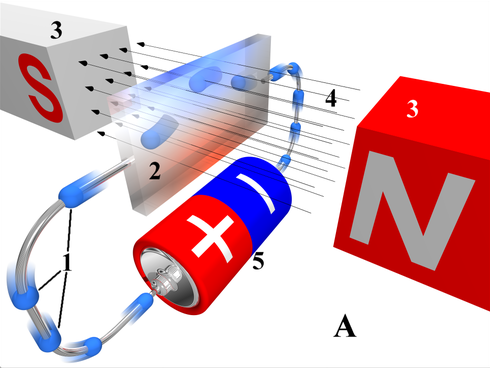
\includegraphics[width = 0.6 \textwidth]{Hall_effect}
		\caption{Пример действия эффекта Холла на свободные заряды}
	\end{center}
\end {figure}



$$\boldsymbol{F_\text{Л}}  = -e \boldsymbol{E} - e \langle \boldsymbol{\upsilon} \rangle \times \boldsymbol{B},$$
где $e$ - абсолютная величина заряда электрона, $\boldsymbol{B}$ - индукция магнитного поля, $\boldsymbol{E}$ - напряженность электрического поля, $ \langle \boldsymbol{\upsilon} \rangle$ - средняя скорость заряда.

Из этого выражения получим разность потенциалов между двумя гранями:

\begin{equation}
U = -E_zl = - | \langle \upsilon \rangle | B l
\label{eq:pot_dif}
\end{equation}

С этой возникшей разностью потенциалов и связан Эффект Холла.

Далее, если выразить ток:
$$ I = ne |\langle \upsilon \rangle |  l a$$
И совместить его с \ref{eq:pot_dif}, получим ЭДС Холла:

\begin{equation}
\mathscr{E}_x = U = - \dfrac{IB}{nea} = -R_x \cdot \dfrac{IB}{a},
\label{eq: Hall}
\end{equation}

где $R_x = \dfrac{1}{ne}$ называется \textit{постоянной Холла.}

\subsection*{Установка и параметры измерения}

\begin{wrapfigure}[14]{l}{0.7 \textwidth}
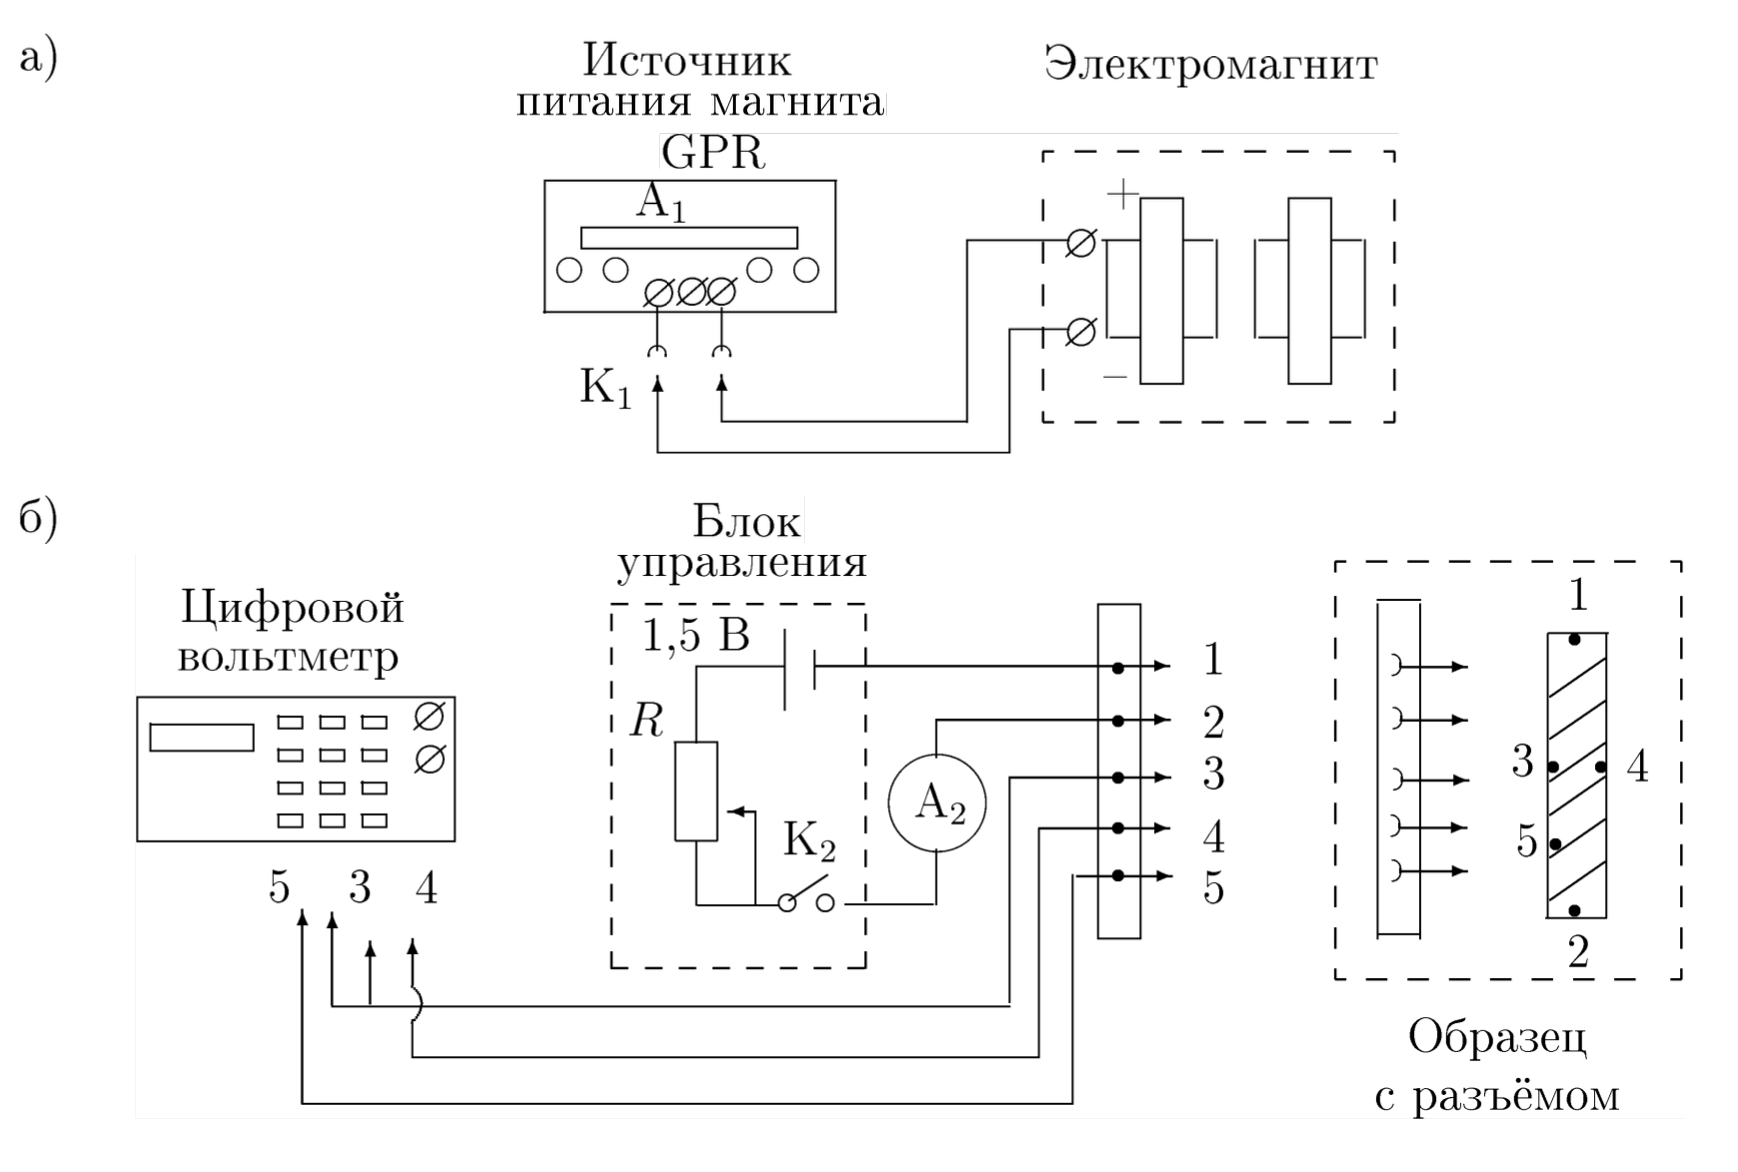
\includegraphics[width = 0.7 \textwidth]{Scheme1.png}
			\caption{Схема установки для измерения эффекта Холла в полупроводниках}
\end{wrapfigure} 

$$\text{Параметры установки:}$$
$$a = 2.2 \text{ мм}$$
$$L_{35} = 3 \text{ мм}$$
$$l = 2.5 \text{ мм}$$
\vspace{5.7 cm}

В нашей установке вдоль длинной стороны образца будет течь ток, величина которого регулируется реостатом $R_2$. Так как он помещен в электромагнит, между точками \textit{3 и 4} будет возникать разность потенциалов $U_{34}$, которую мы будем измерять. 

Однако между точками \textit{3 и 4} будет возникать некоторое дополнительное падение напряжения $U_{0}$, так как эти точки оказываются не на одной эквипотенциали. Исключить это влияние можно с помощью изменения направления магнитного поля: в одном случае $U_{34} = U_{0} - \mathscr{E}_x $, в другом  $U_{34} = U_0 - \mathscr{E}_x $. Тогда с помощью полуразности избавимся от $U_{0}$ в наших измерениях. 

\begin{figure}[H]
	\begin{center}
		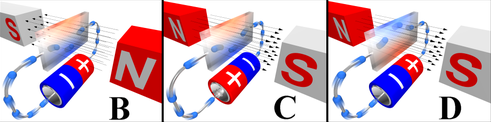
\includegraphics[width = 0.6 \textwidth]{Hall_dif}
		\caption{Эффект Холла при различных направлениях магнитного поля и тока через образец}
	\end{center}
\end{figure}

\section{Работа и измерения}

\paragraph{Калибровка установки}
Во время проведения работы, мы сняли зависимость магнитного потока $\varPhi$ от силы тока $I$, так же нам известно, что $\varPhi=BSN$, где $SN=75\text{ см}^2\cdot\text{вит}$.
\begin{table}[H]
\centering
\caption{Данные для калибровки установки}
\begin{tabular}{c|c c c c c c c c}
\toprule
$I, \text{ мА}$ & 0.20    & 0.33   & 0.44 & 0.57   & 0.69   & 0.87 & 1.00     & 1.15   \\
$\varPhi, \text{ мВб}$ & 2.3 & 2.9 & 3.4 & 4.0 & 4.5 & 5.2 & 5.7 & 6.2  \\ \midrule
$B, \text{ Тл}$ & 0.31 & 0.39 & 0.45 & 0.53 & 0.60 & 0.69 & 0.76 & 0.83 \\ \bottomrule
\end{tabular}
\label{calibrate}
\end{table}

	\begin {figure}[H]
	\label{graph1}
		\begin{center}
			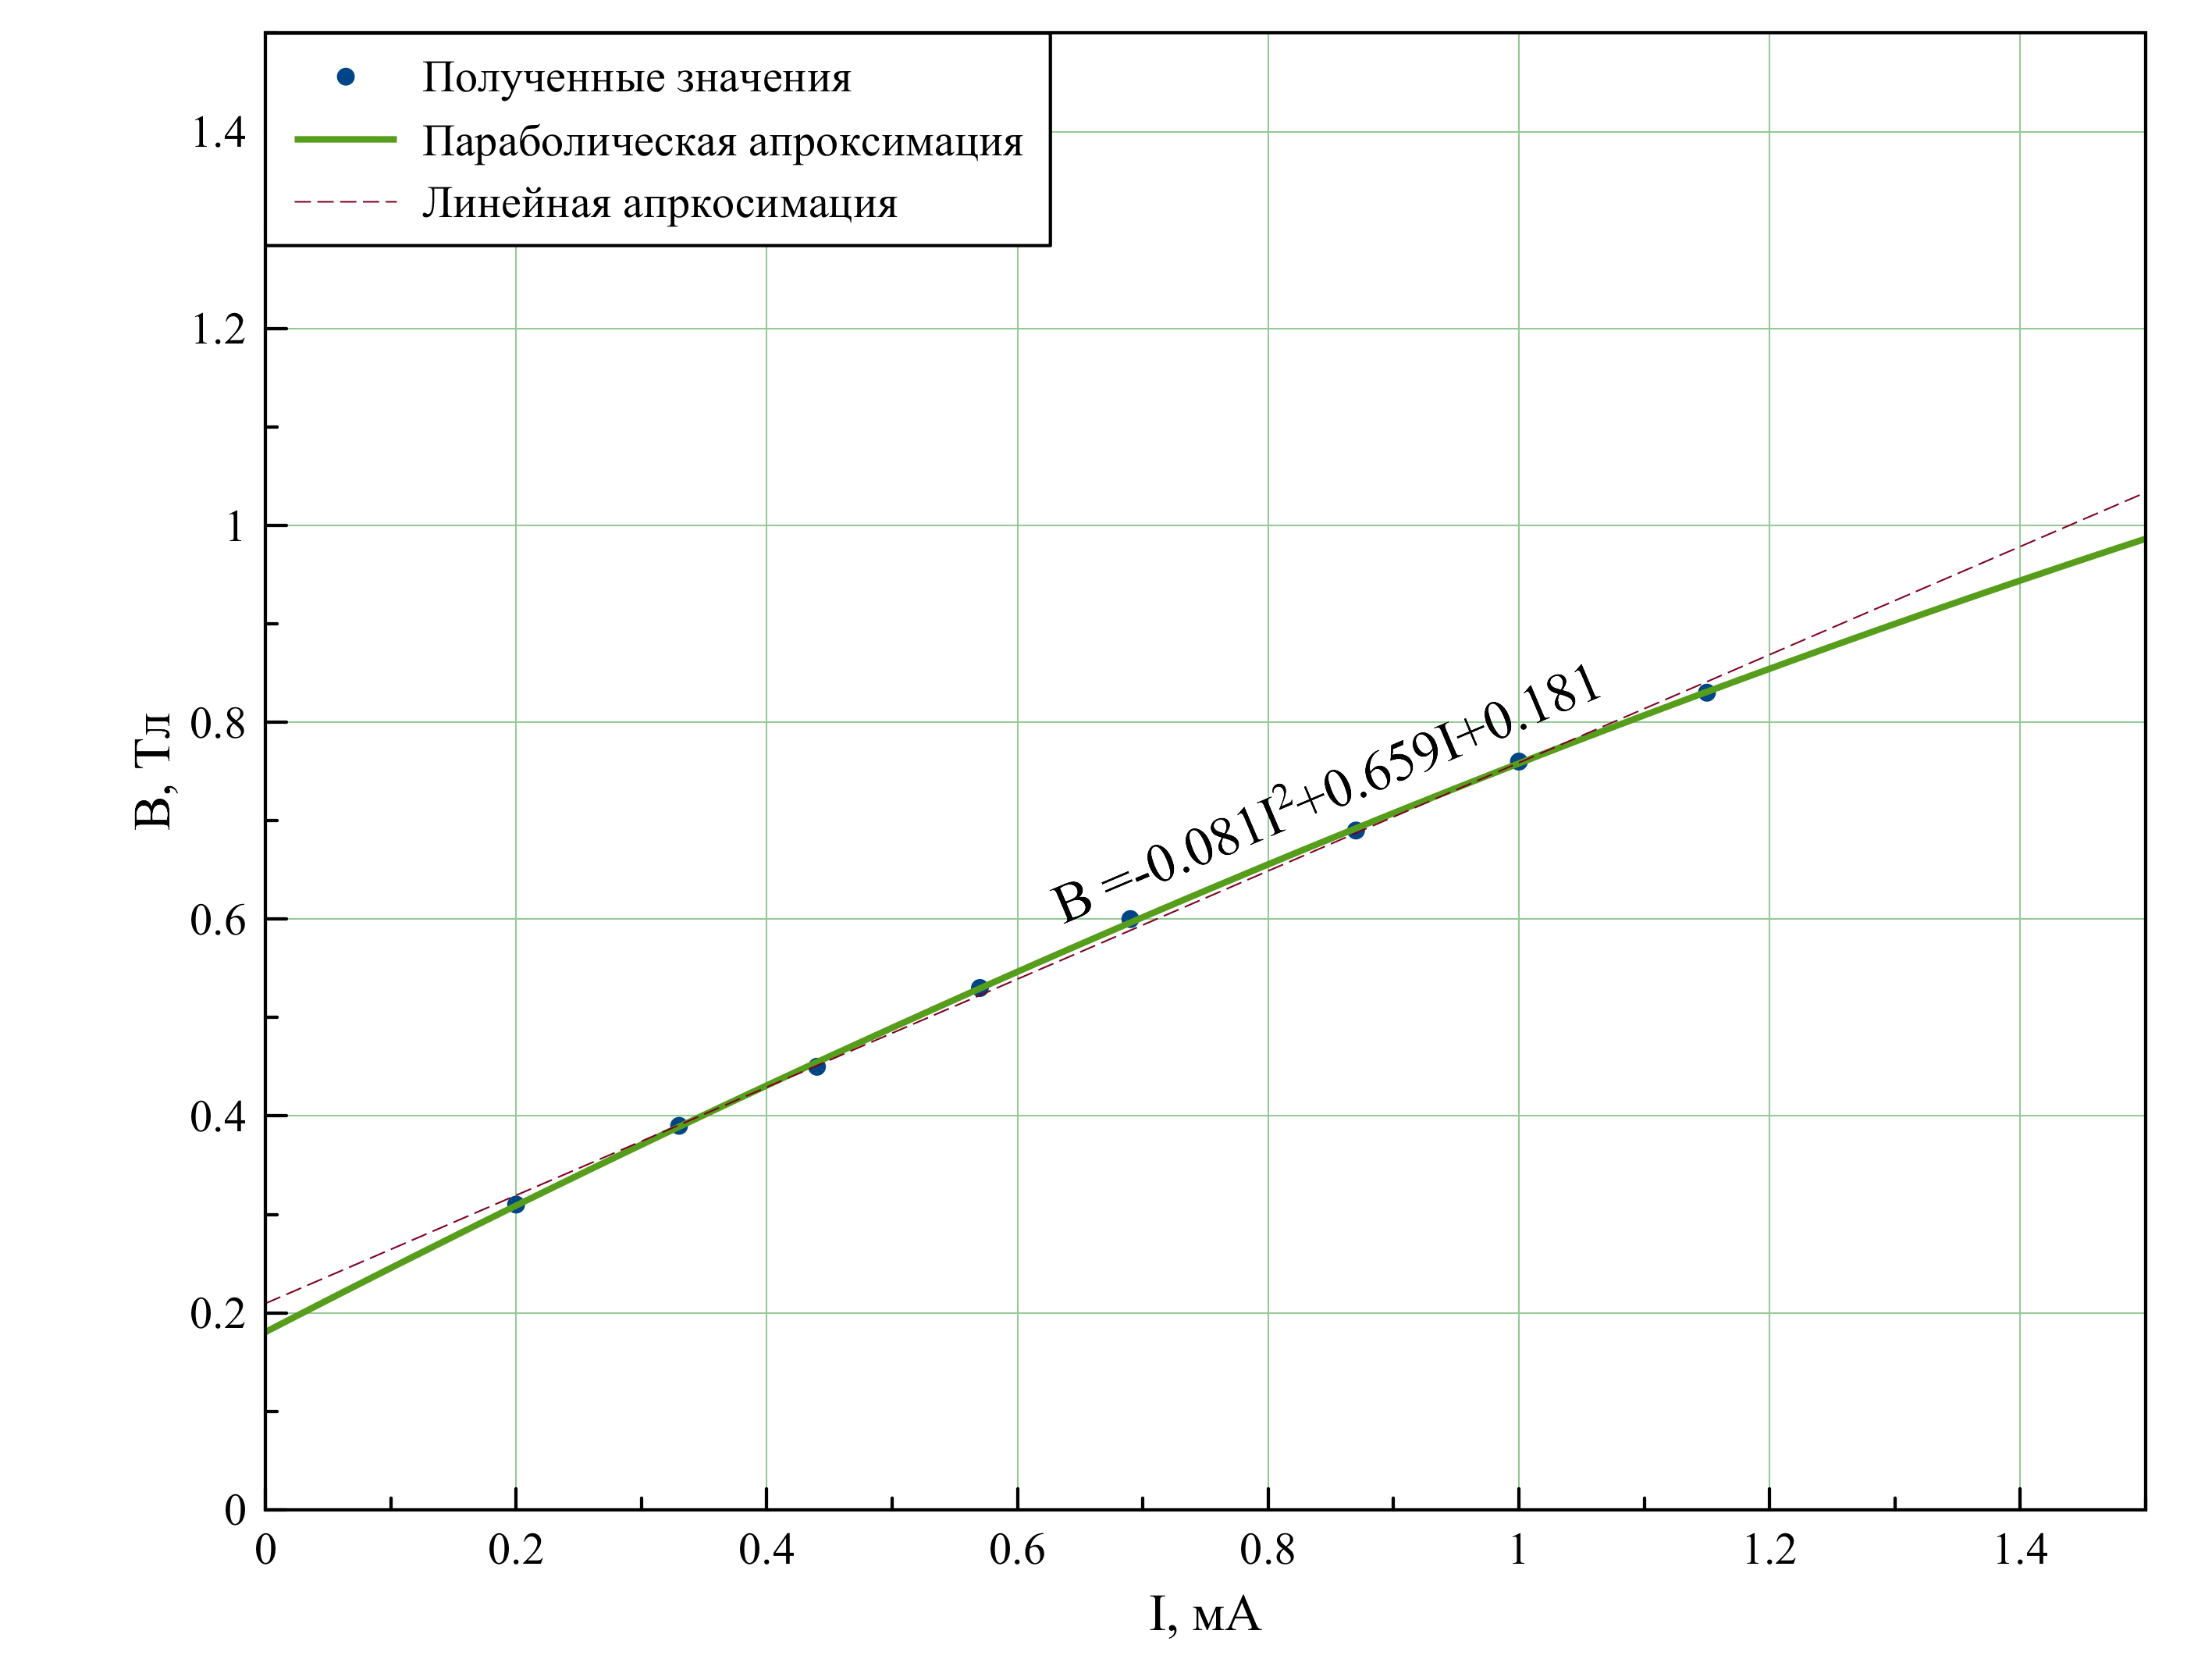
\includegraphics[width = 0.9 \textwidth]{graph1.png}
			\caption{Калибровка установки}
		\end{center}
	\end {figure}
Как можно видеть по графику, параболическая аппроксимация лучше описывает полученную зависимость чем линейная. Из этого можно сделать вывод о том, что индукция зависит от тока параболически . С помощью рабочей среды Anaconda вычислим зависимость, $B = -0,081\cdot I^2+0,659\cdot I+0,181$

\begin{table}[H]
	\centering
	\label{my-label}
	\caption{Зависимость ЭДС Холла от магнитного поля}
	\begin{tabular}{c|c|c|c|c|c|c|c|c|c|c}
		\toprule
		\multirow{2}{*}{$I, \text{ мА}$} & \multirow{2}{*}{$U_0, \text{ мВ}$} & $I_M, \text{ мА}$                                                      & 0.2    & 0.4    & 0.6    & 0.9    & 1.2    & 1.5   & 1.8    & 2.1    \\% \cline{3-11}
		&                                    & $B, \text{ Тл}$                                                        & 0.309  & 0.431  & 0.547  & 0.708  & 0.854  & 0.986  & 1.104  & 1.207  \\ \midrule
		\multirow{2}{*}{0.3}             & \multirow{2}{*}{0.010}              & $U, \text{мВ}$                                                         & 0,001  & -0.006 & -0.014 & -0.021 & -0.029 & -0.036 & -0.044 & -0.049 \\% \cline{3-11} 
		&                                    & \begin{tabular}[c]{@{}c@{}}$\mathscr{E}_x,$  $ \text{мВ}$\end{tabular} & -0.009 & -0.016 & -0.024 & -0.031 & -0.039 & -0.046 & -0.054 & -0.059 \\ \midrule	
		\multirow{2}{*}{0.4}             & \multirow{2}{*}{0.012}             & $U, \text{мВ}$                                                         & 0.002  & -0.007 & -0.019 & -0.034 & -0.047 & -0.057 & -0.062 & -0.067 \\% \cline{3-11} 
		&                                    & \begin{tabular}[c]{@{}c@{}}$\mathscr{E}_x,$   $\text{мВ}$\end{tabular} & -0.010 & -0.019 & -0.031 & -0.046 & -0.059 & -0.069 & -0.074 & -0.079 \\ \midrule
		\multirow{2}{*}{0.5}             & \multirow{2}{*}{0.016}             & $U, \text{мВ}$                                                         & 0.003  & -0.010 & -0.022 & -0.041  & -0.058 & -0.070 & -0.079 & -0.083 \\% \cline{3-11} 
		&                                    & \begin{tabular}[c]{@{}c@{}}$\mathscr{E}_x,$   $\text{мВ}$\end{tabular} & -0.013 & -0.026 & -0.038 & -0.057  & -0.074 & -0.086 & -0.095 & -0.099 \\ \midrule
		\multirow{2}{*}{0.6}             & \multirow{2}{*}{0.019}             & $U, \text{мВ}$                                                         & 0.004  & -0.013 & -0.027 & -0.050 & -0.069 & -0.083 & -0.093 & -0.098 \\% \cline{3-11} 
		&                                    & \begin{tabular}[c]{@{}c@{}}$\mathscr{E}_x,$ $ \text{мВ}$\end{tabular} & -0.015 & -0.032 & -0.046 & -0.069 & -0.088 & -0.102 & -0.112 & -0.117 \\ \midrule
		\multirow{2}{*}{0.7}             & \multirow{2}{*}{0.023}             & $U, \text{мВ}$                                                        & 0.006  & -0.012 & -0.031 & -0.057 & -0.081 & -0.097 & -0.109 & -0.114 \\% \cline{3-11} 
		&                                    & \begin{tabular}[c]{@{}c@{}}$\mathscr{E}_x,$   $\text{мВ}$\end{tabular} & -0.017 & -0.035 & -0.054 & -0.080 & -0.104 & -0.120 & -0.132 & -0.137 \\ \midrule
		\multirow{2}{*}{0.8}             & \multirow{2}{*}{0.027}             & $U, \text{мВ}$                                                         & 0.005  & -0.015 & -0.035 & -0.065 & -0.091 & -0.110 & -0.123 & -0.130 \\% \cline{3-11} 
		&                                    & \begin{tabular}[c]{@{}c@{}}$\mathscr{E}_x,$  $ \text{мВ}$\end{tabular} & -0.022 & -0.042 & -0.062 & -0.092 & -0.118 & -0.137 & -0.150 & -0.157 \\ \midrule
		\multirow{2}{*}{0.9}             & \multirow{2}{*}{0.029}             & $U, \text{мВ}$                                                          & 0.007  & -0.016 & -0.039 & -0.073 & -0.103 & -0.124 & -0.140 & -0.147 \\% \cline{3-11} 
		&                                    & \begin{tabular}[c]{@{}c@{}}$\mathscr{E}_x,$  $\text{мВ}$\end{tabular}& -0.022 & -0.045 & -0.068 & -0.102 & -0.132 & -0.153 & -0.169 & -0.176 \\ \midrule
		\multirow{2}{*}{1.0}               & \multirow{2}{*}{0.033}             & $U, \text{мВ}$                                                        & 0.009  & -0.017 & -0.044 & -0.081 & -0.114 & -0.138 & -0.154 & -0.162 \\% \cline{3-11} 
		&                                    & \begin{tabular}[c]{@{}c@{}}$\mathscr{E}_x,$  $\text{мВ}$\end{tabular} & -0.024 & -0.050 & -0.077 & -0.114 & -0.147 & -0.171 & -0.187 & -0.195 \\ \midrule
		\multirow{2}{*}{1.0}               & \multirow{2}{*}{0.040}              & $U, \text{мВ}$                                                         & 0.065  & 0.092  & 0.118  & 0.155  & 0.189  & 0.213  & 0.229  & 0.237  \\% \cline{3-11} 
		&                                    & \begin{tabular}[c]{@{}c@{}}$\mathscr{E}_x,$ $ \text{мВ}$\end{tabular} & 0.025  & 0.052  & 0.078  & 0.115  & 0.149  & 0.173  & 0.189  & 0.197  \\ \bottomrule[0.65mm]
	\end{tabular}
\end{table}
Опять же заметим, что гиперболическая аппроксимация сильнее удовлетворяет полученным значениям, но из расчетов данных из таблицы \ref{calibrate} видно, что вклад квадратичной составляющей невелик, поэтому будем анализировать полученные данные с помощью МНК. Отобразим их в таблице \ref{my-label}.
\begin{table}[H]
	\centering
	\caption{Зависимость углового коэффициента от силы тока}
	\label{my-label}
	\begin{tabular}{c|c c c c c c c c}
		\toprule
		$I, \text{ мА}$                                           & 0.3    & 0.4    & 0.5    & 0.6    & 0.7    & 0.8    & 0.9    & 1.0    \\
		$k,\,\text{мВ}\cdot\text{Тл}\slash\text{мА}$          & -0.055 & -0.080 & -0.100 & -0.118 & -0.140 & -0.157 & -0.179 & -0.199 \\ \midrule
		$\sigma_k\,\text{мВ}\cdot\text{Тл}\slash\text{мА}$ & 0.001  & 0.003  & 0.004  & 0.005  & 0.006  & 0.006  & 0.007  & 0.008  \\ \midrule
		$\sigma_I, \text{ мА}$                                 & \multicolumn{8}{c}{0,01}                                             \\ \bottomrule
	\end{tabular}
\end{table}
Также изобразим эти данные на графике (Рис. 6). Опять же с помощью МНК получаем, что $$K = -(0.202\pm 0.002)\dfrac{\text{мкВ} \cdot \text{Тл}}{\text{мА}}$$
Из формулы (2) посчитаем постоянную Холла:
$$R_x = \dfrac{\mathscr{E}_x}{IB} \cdot a = - K \cdot a = (444 \pm 4) \cdot 10^{-6}\; \text{ м}^3\slash\text{Кл}$$
	\begin {figure}[H]
		\begin{center}
			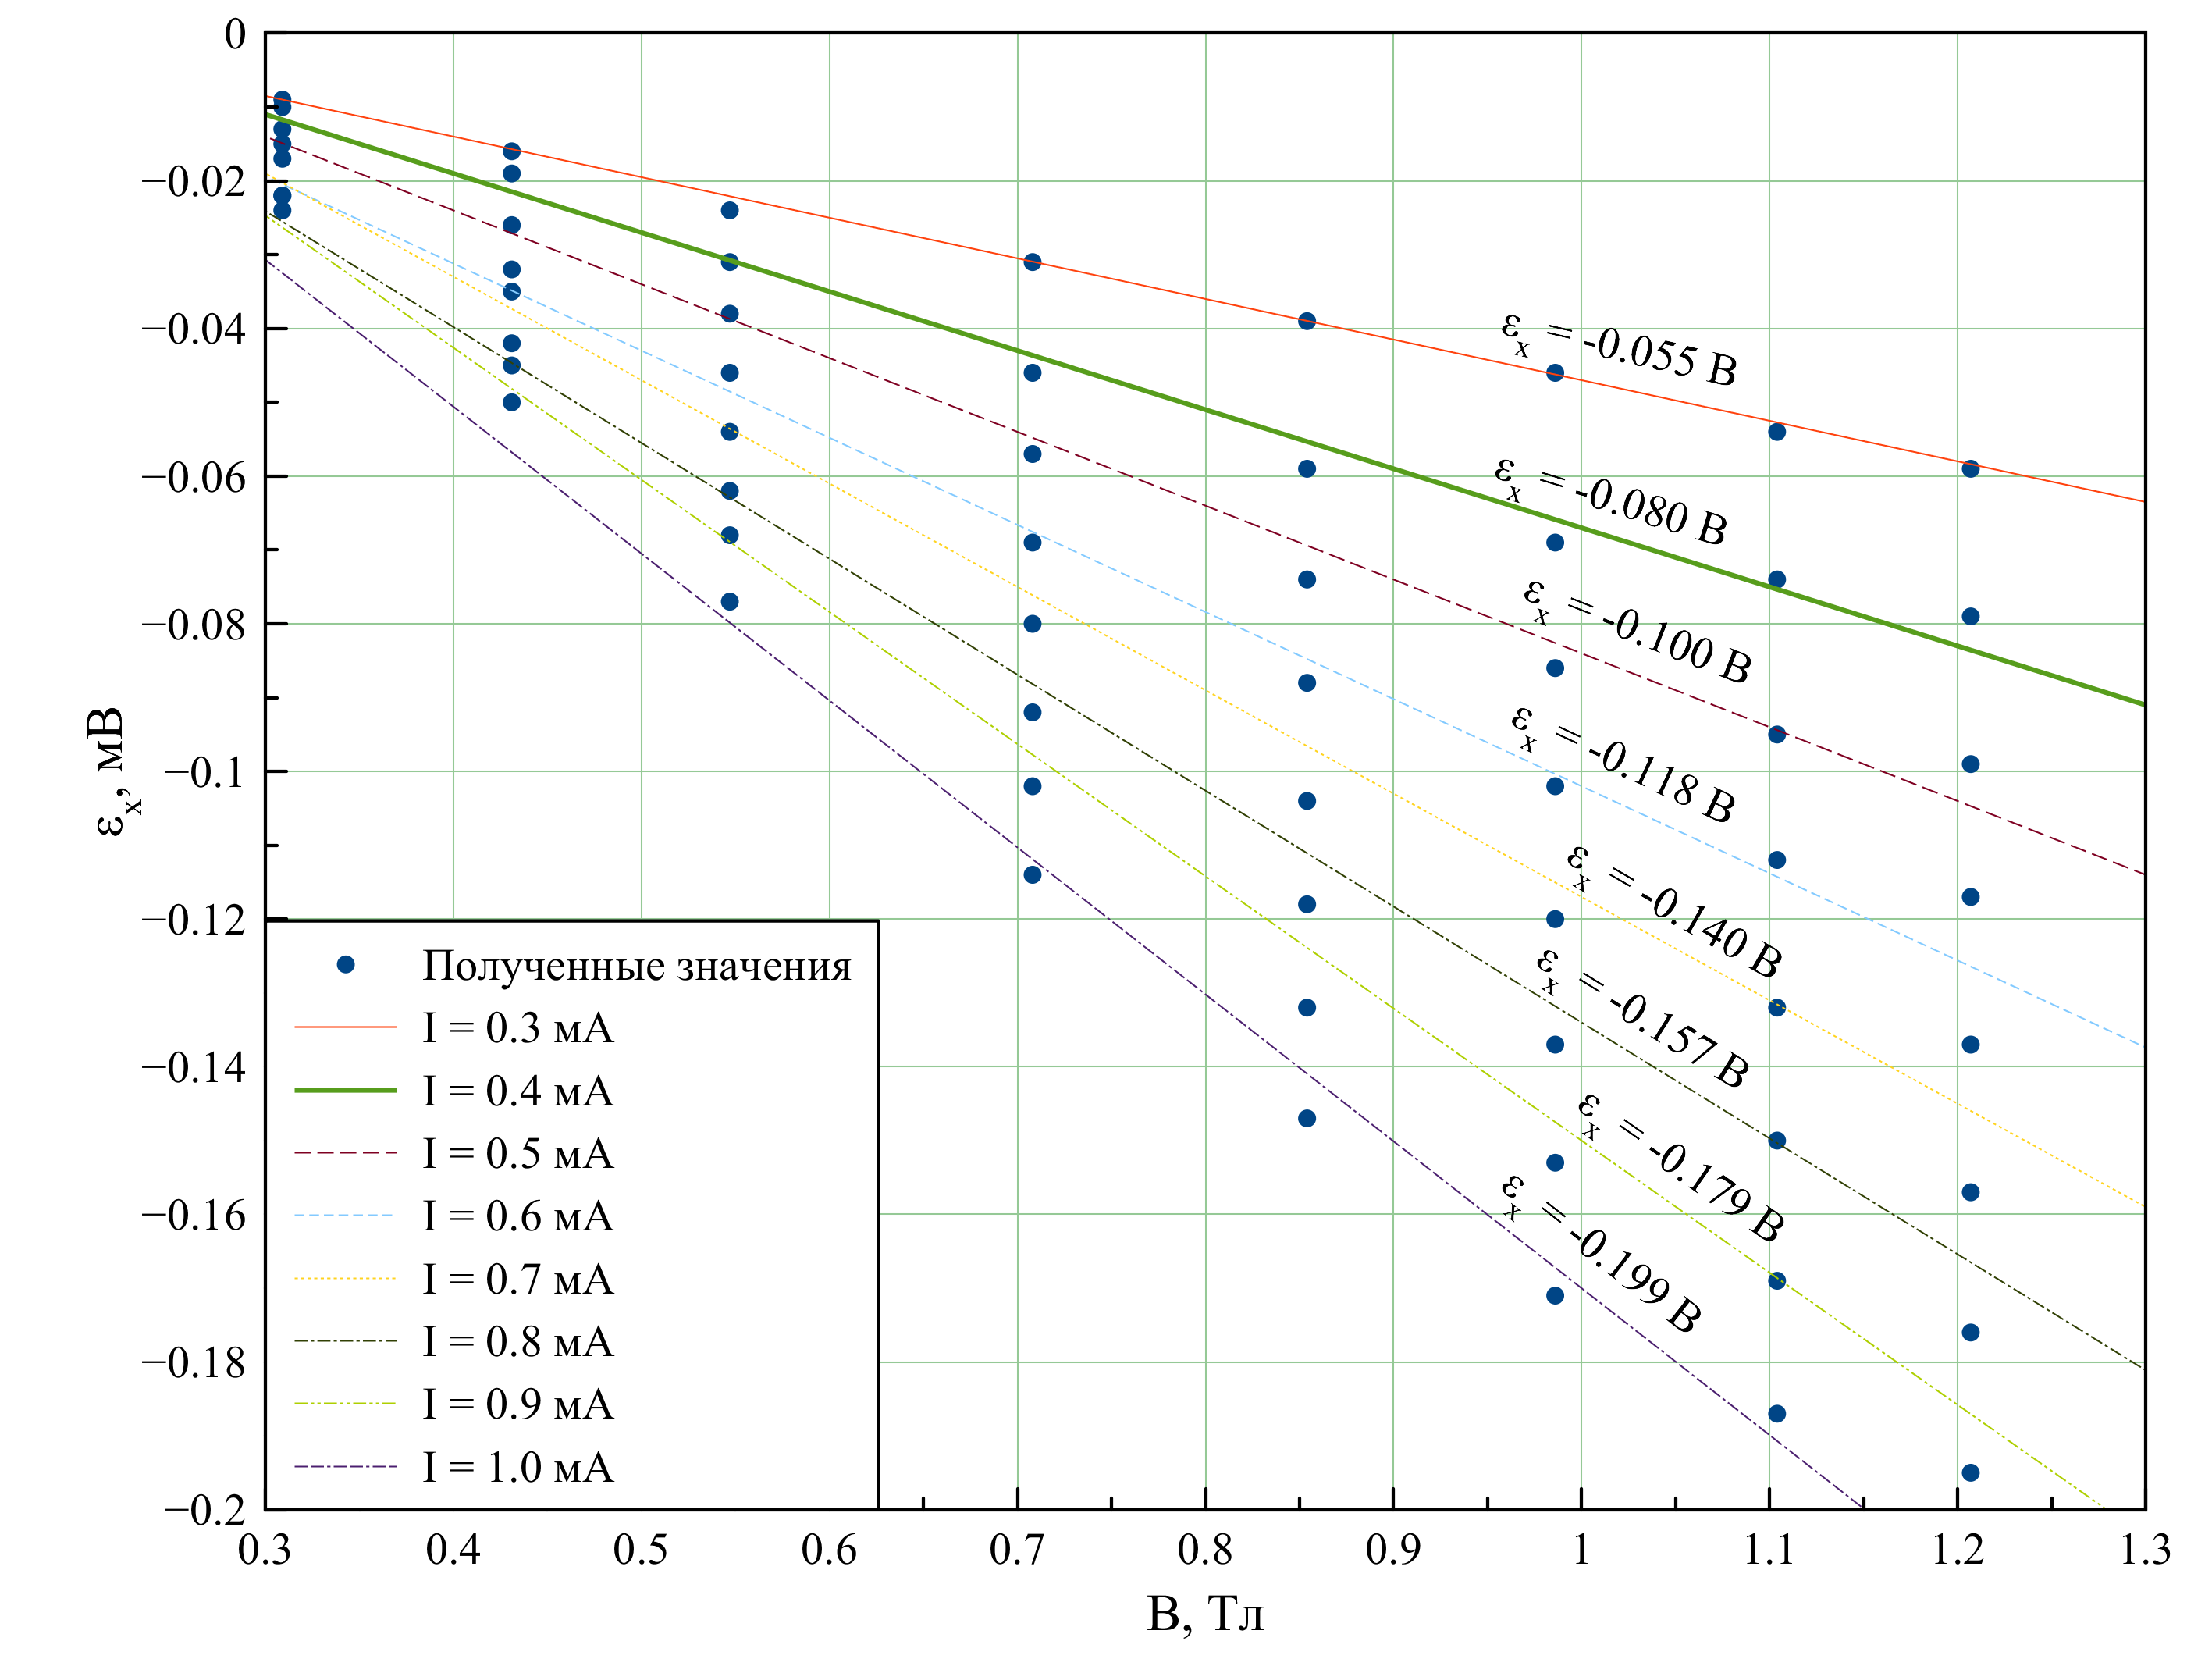
\includegraphics[width = 0.9 \textwidth]{graph2.png}
			\caption{график зависимости $\mathscr{E}_x = f(B)$ для разных $I$}
		\end{center}
	\end {figure}
	
		\begin {figure}[H]
	\begin{center}
		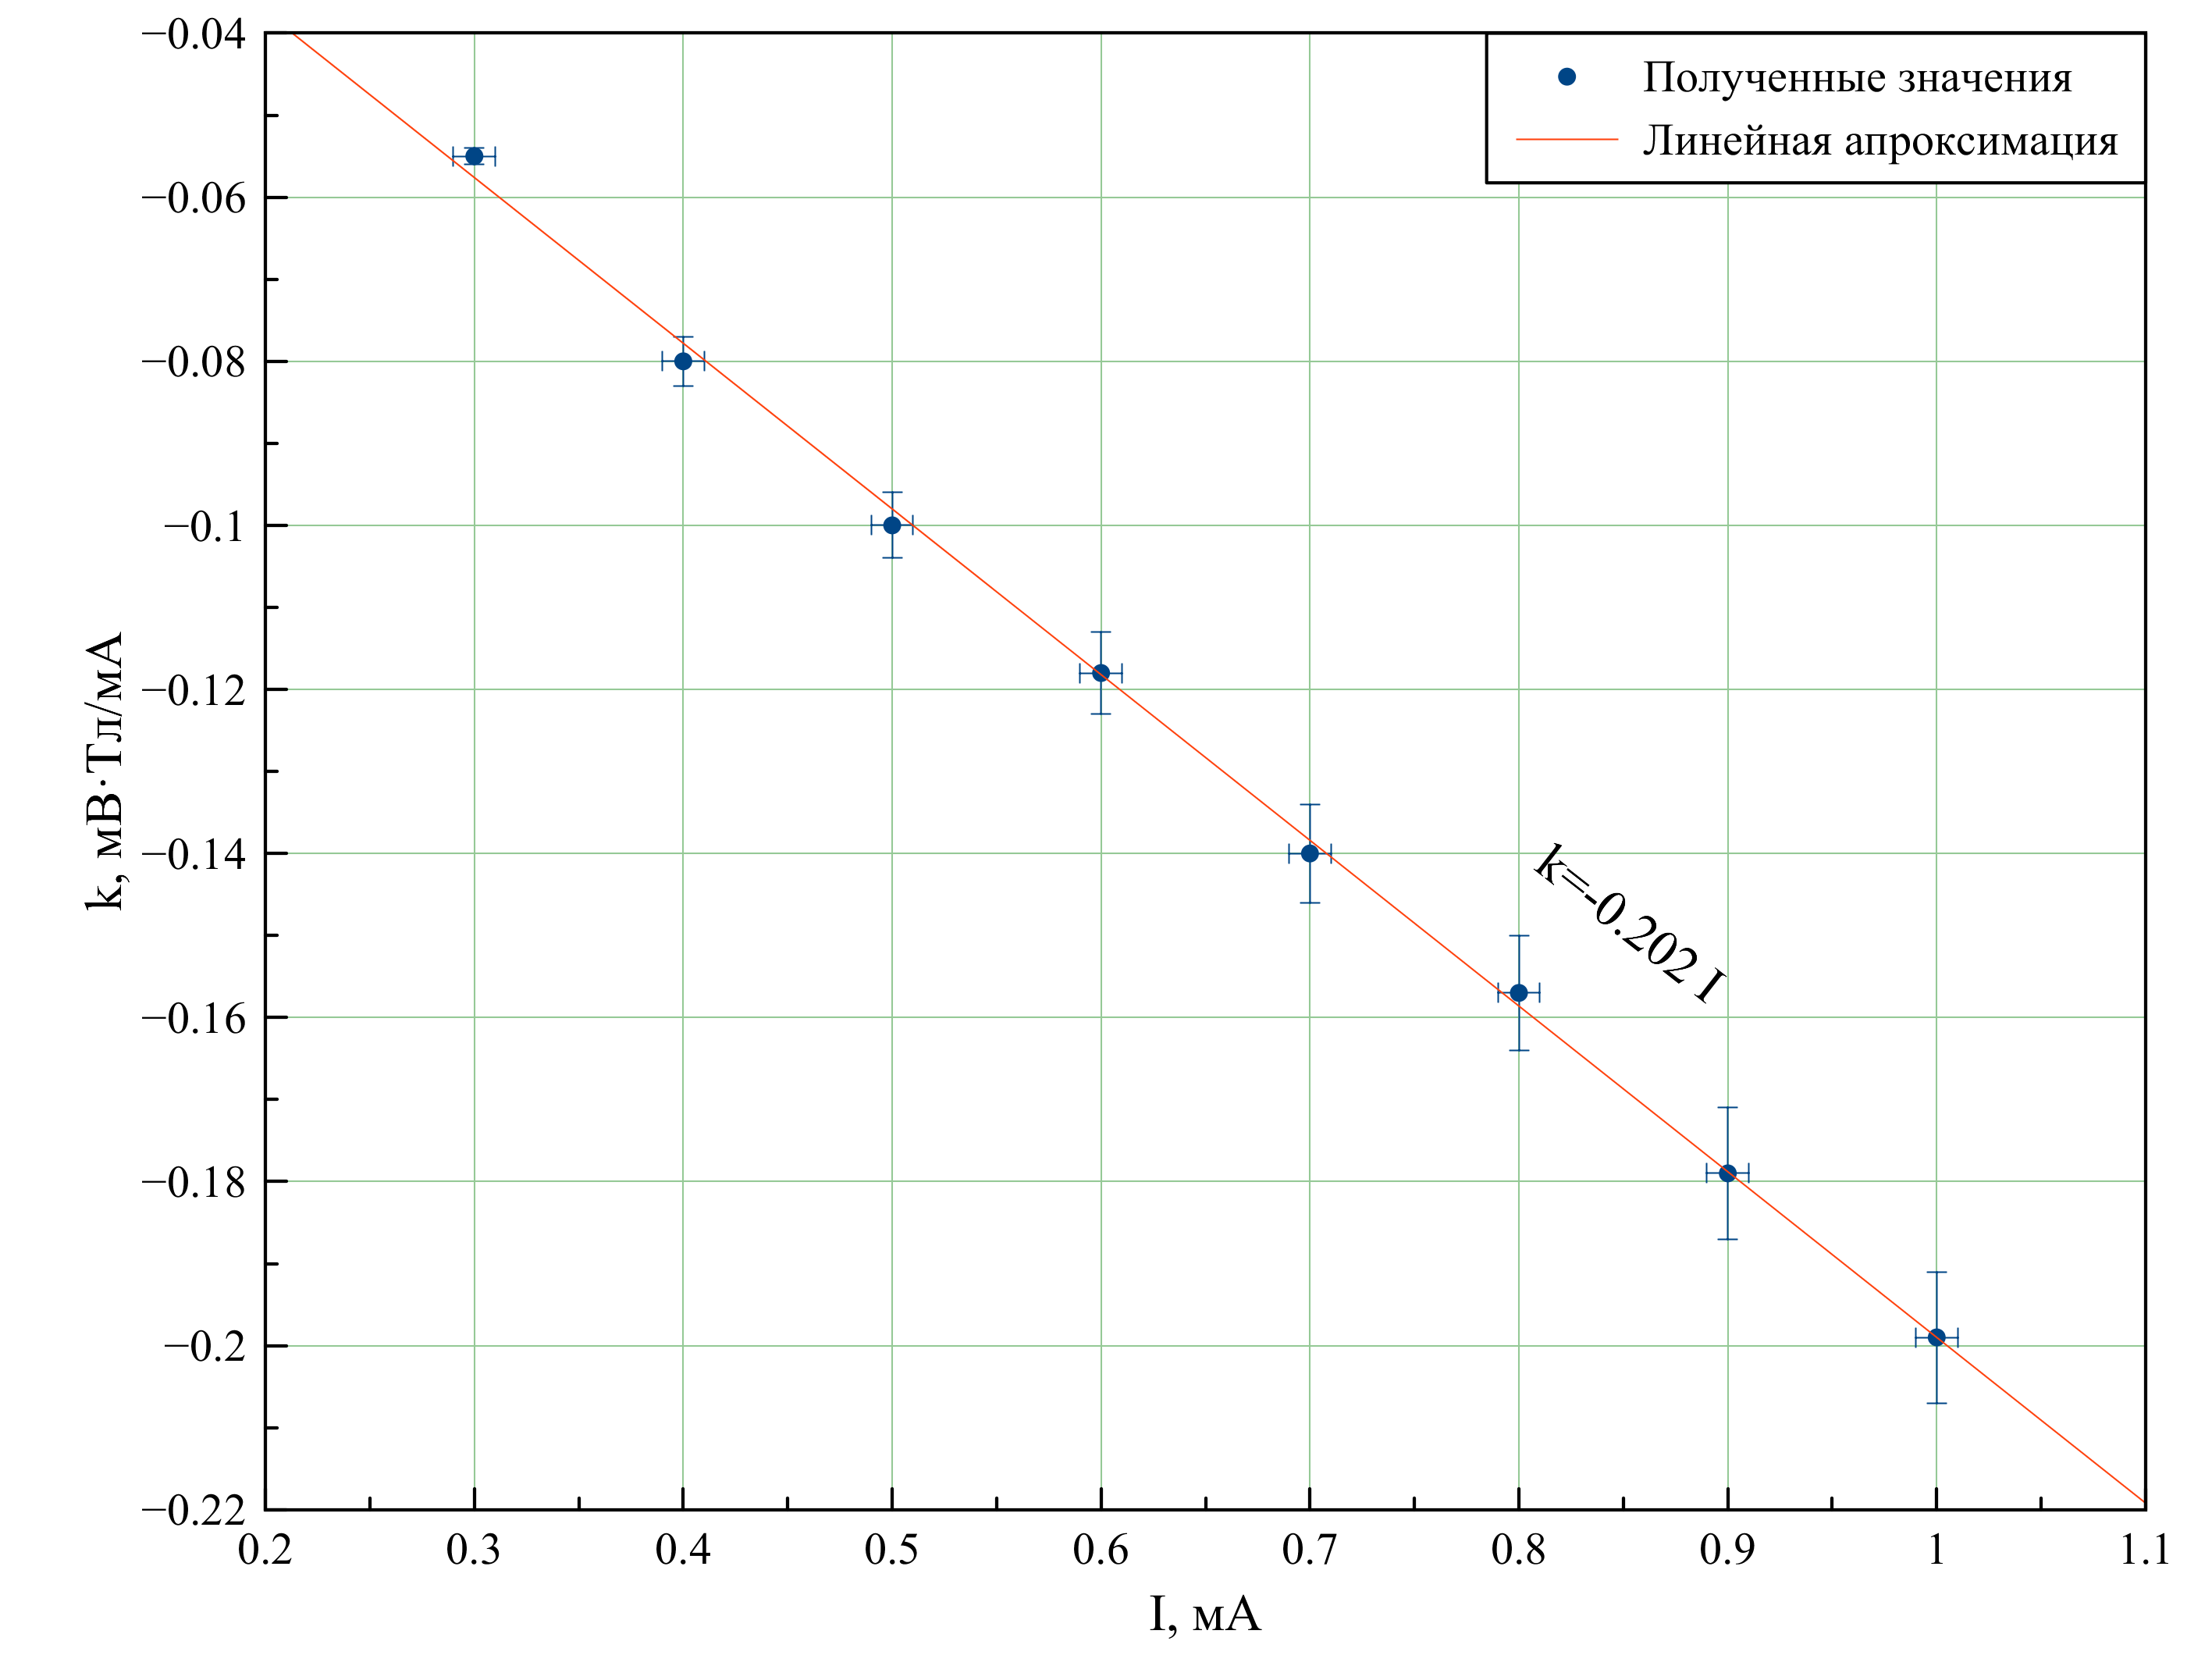
\includegraphics[width = 0.85 \textwidth]{graph3.png}
		\caption{График зависимости углового коэффициента от силы тока}
	\end{center}
	\end {figure}

Определим концентрацию носителей заряда: $n = \dfrac{1}{eR_x} = (1.4 \pm 0.2) \cdot 10^{22} \; 1/\text{м}^3$
	
Вычислим удельную проводимость материала с помощью $U_{35}=1.735$ мВ: $$\sigma=\dfrac{I L_{35}}{U_{35} al} =314\pm3(\text{Ом}\cdot\text{м})^{-1}$$

Рассчитаем подвижность электрона:
$$b = \dfrac{\sigma}{en} = 1.4 \cdot 10^{3}\,\dfrac{\text{см}^2}{\text{В} \cdot \text{с}},\quad \Delta b=b\cdot\sqrt{\varepsilon_\sigma^2+\varepsilon_n^2}=0.2\cdot 10^{3}\,\dfrac{\text{см}^2}{\text{В} \cdot \text{с}}$$

\section{Вывод}

Мы определили постоянную Холла для германия. Полученная проводимость n-типа. Измерили подвижность и концентрацию заряда в полупроводниках.

\end{document}
